% -*- root: ../thesis.tex -*-
%!TEX root = ../thesis.tex
% ******************************* Thesis Chapter 1 ****************************

% ----------------------------------------------------------------------
%: ----------------------- introduction content ----------------------- 
% ----------------------------------------------------------------------

% ----------------------- paths to graphics ------------------------

% change according to folder and file names
\graphicspath{{1_introduction/figures/}}
% ----------------------- contents from here ------------------------

The realm of web applications that companies are offering has grown in the last decades to a point where they are essential for our society to function. Although it has brought many advantages, a big problem with this development is how personal data are collected and used. In particular, the business model of many tech companies is to collect and sell data.
For example, large online platforms use personal data linked to a natural person, such as age, gender, interests, and many more, to advertise products. This model is called personalized advertising \cite{tucker_social_2014}. Since these practices limit individual freedom and privacy, many countries have started adopting laws. A relevant regulation for this thesis is the GDPR \cite{noauthor_general_2016}, which applies to the European Union. With its implementation in 2018, many new challenges for companies came up with adopting the requirements.
In this thesis, we aim to integrate Transparency Enhancing Technologies into Cloud-Native Infrastructures to foster Transparency in systems and to meet regulatory givens.

\section{Cloud-Native Systems}
Many modern web applications are complex because they have to fulfill a variety of requirements. 
To realize a rich set of features, the source code of these applications tends to grow bigger and bigger. When everything is written in one codebase and deployed as one instance - a monolithic design, this practice can result in some problems. For example, coordination between big teams can be impacted, updating simple features requires the whole application to be redeployed, or searching for errors can be complicated. Because of this and some other qualities, like scalability, the Microservice architecture is often used today \cite{alshuqayran_systematic_2016}. It is based on service-oriented architecture and requires the application to be split into multiple services. Each service realizes a discrete functionality and exposes an interface for communicating with other services. 


Another modern development is the usage of cloud platforms and, therefore, the adoption of PaaS (Platform as a Service). One of the most popular PaaS technologies is Kubernetes, which allows for the abstraction of applications and services into units called Pods. The difference between the previously used Virtual machines in Infrastructure as a Service is the decoupling of the running application instance from the physical server. Besides this, Kubernetes allows mechanisms to scale Pods and ensure availability across different physical servers and data centers. This uprise in popularity went hand-in-hand with the adoption of Microservices \cite{hardikar_containerization_2021}.

\begin{figure}[!htb]
  \centering
  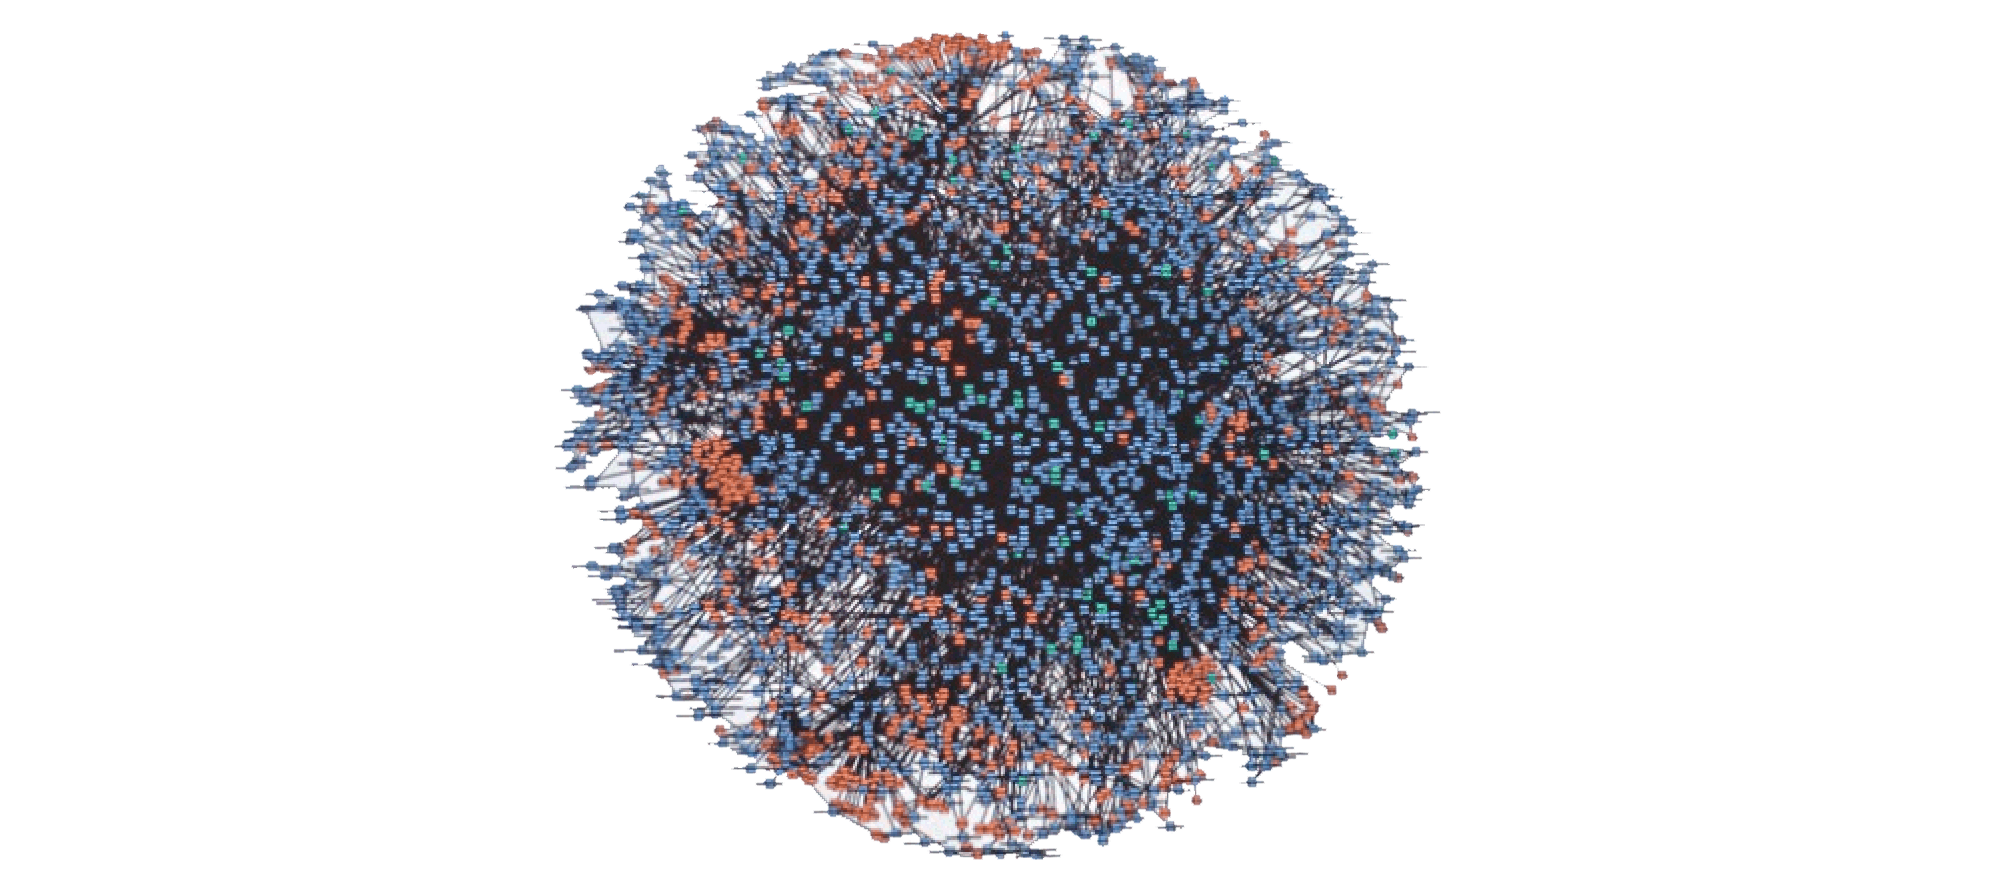
\includegraphics[width=0.95\columnwidth]{amazon.png}
  \caption[Amazon Architecture]{Microservice architecture of Amazon.com \footnote{\url{https://www.sayonetech.com/blog/5-microservices-examples-amazon-netflix-uber-spotify-and-etsy/}}}  
  \label{fig:amazon-arch}
\end{figure}

The service graph shown in figure \ref{fig:amazon-arch} displays the architecture of the Amazon\footnote{\url{https://amazon.com}} Website and App.
Each dot represents a service, and the lines between the dots represent a connection. The communication happens over standardized APIs. A Microservice architecture often requires services to communicate with each other to realize certain features. However, it should be noted that Amazon.com has a reasonably complex architecture and that many other companies have far less complexity.

\begin{figure}[!htb]
  \centering
  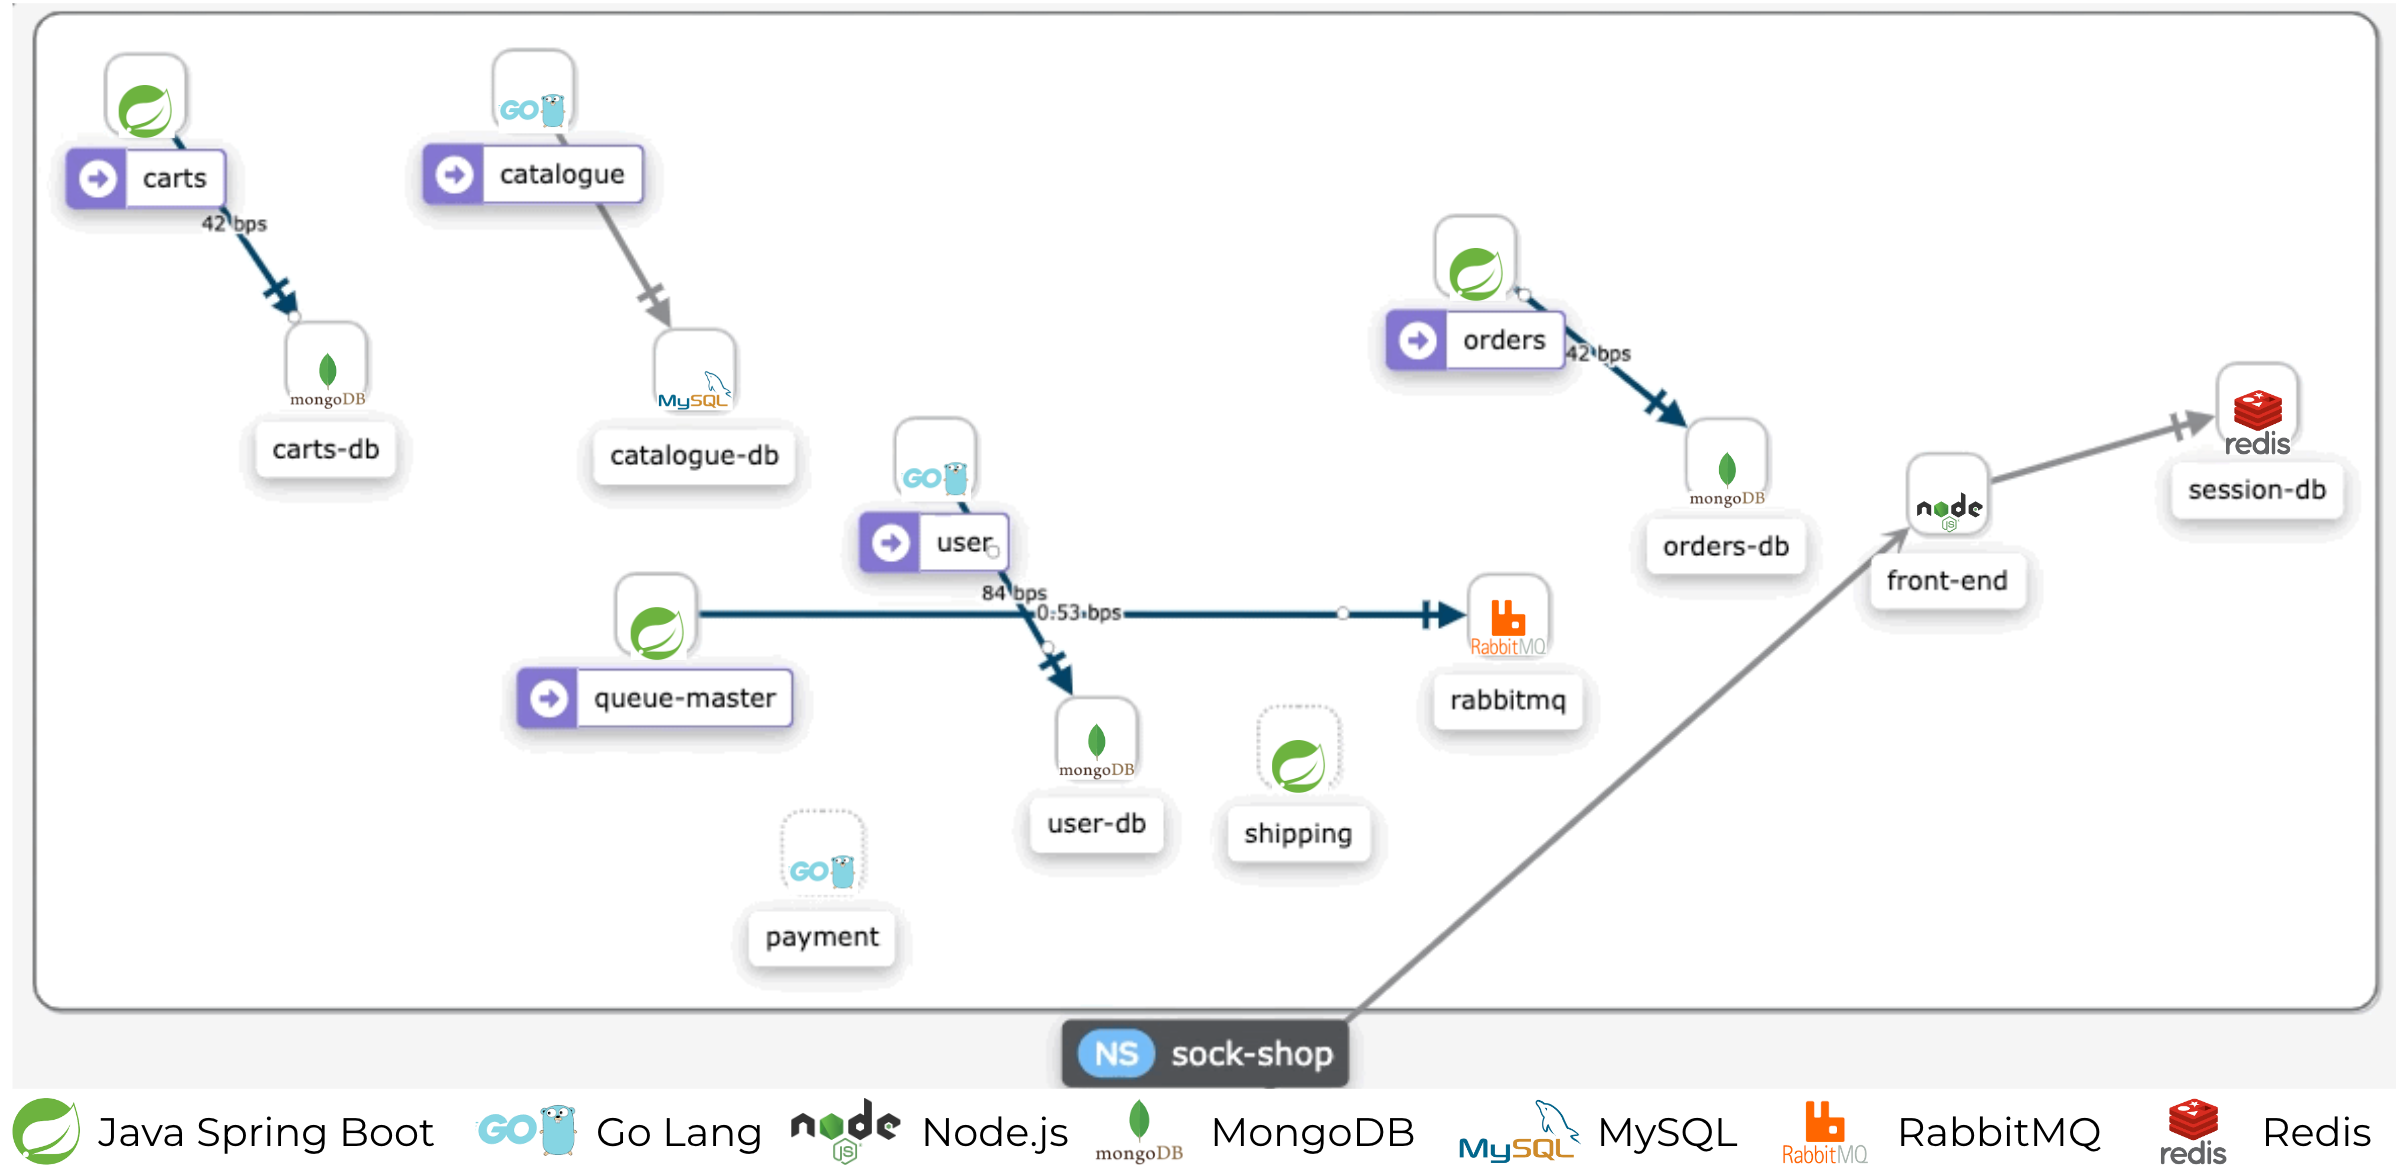
\includegraphics[width=0.95\columnwidth]{sockshop.png}
  \caption[Sockshop Architecture]{Demo Microservice architecture Sock Shop. \footnote{\url{https://github.com/microservices-demo/microservices-demo}}} 
  \label{fig:sockshop-arch}
\end{figure}

A much simpler Microservice architecture can be found in figure \ref{fig:sockshop-arch}. The Sock Shop project, developed by Weaveworks \footnote{\url{https://www.weave.works/}}, is designed to act as a placeholder for a typical (small) online shop. 
Compared to the Amazon.com architecture, it is much more apparent which service communicates with which, although it should be noted that this graph is not quite complete because typically, the front-end, e.g., the user-agent, would communicate with all of them. There are also some cases present where inter-service communication happens in this example. However, we indicate that icons suffixed with \texttt{db} stand for \texttt{database}. Note that databases are mostly not services for themselves, although they might be in separate Pods in the case of Kubernetes. Instead, they contribute to a service that can internally consist of multiple different programs. For example, the \texttt{carts-service} consists of two programs, namely, \texttt{carts}, a program written in Java Spring Boot and a \texttt{carts-db} with MongoDB as a database for persistence behind it. Since services should expose a defined interface, typically using restful HTTP, the database is often excluded from the interface specification.


From a privacy perspective, this means that data, more importantly, personal data, might be stored at and across many different databases. Monitoring which database contains which data is getting much more complicated than having, e.g., one extensive database with all application data in it. This is especially bad when services save parts of data from other services. Now by imagining this at a scale like Amazon, this problem extends even further.

\section{Legal background}
As mentioned in the sections above, the main regulatory framework of this thesis is the GDPR because it is applicable in the EU.
The GDPR regulates how companies and public institutions collect and process personal data. Personal data means information that can be linked to an identifiable person. A big challenge for companies is Article 13 and the following, which are described in depth in a later section. These articles require companies/institutions to disclose what personal data is stored and processed. 

\section{Transparency Enhancing Technologies}
Now, to tie on to the data transparency problem described in the sections above, a new group of technologies gained popularity - the so-called Transparency Enhancing Technologies (TET). Many such technologies are already available, which help inspect the data flow inside a modern application. One example is Google Cloud Data Loss Prevention\footnote{\url{https://cloud.google.com/dlp}}.
Also, more generic privacy-enhancing technologies embody basic data protection principles. Google Differential Privacy, for example, encourages the anonymization of personal data\footnote{\url{https://github.com/google/differential-privacy}}.
However, overall, the usage of all of these technologies is pretty low.


Particularly relevant in this context are the following three groups of technical measures:


\textbf{Data loss prevention (DLP)} describes a whole suite of technologies that detect potential data breaches and/or identify security risks, like, for example, unencrypted passwords, etc. The latter is achieved by scanning data sources like storage buckets, databases, etc. for specific information \cite{zhang_what_2020}. From technology to technology, the information which is searched for can vary. In most cases, it is personal data or passwords. This feature is called data inspection \cite{kim_sensitive_2020}. Many DLP technologies support data inspection directly in their API. The result often contains a list of findings, which is supported by a so-called info type (e.g., email, credit card number) that abstracts the type of data found. \footnote{\url{https://cloud.google.com/dlp/docs/reference/rpc/google.privacy.dlp.v2?hl=de\#google.privacy.dlp.v2.Finding}}\footnote{\url{https://docs.aws.amazon.com/macie/latest/APIReference/findings-describe.html}} Some DLPs also have a risk analysis feature that calculates privacy guarantees such as k-anonymity \cite{sweeney_k-anonymity_2002} or l-diversity \cite{machanavajjhala_l_2007}.\footnote{\url{https://cloud.google.com/dlp/docs/reference/rpc/google.privacy.dlp.v2?hl=de\#analyzedatasourceriskdetails}} Some examples include Google Cloud DLP, AWS Macie\footnote{\url{https://aws.amazon.com/de/macie/}} from industry, and Teiresias from academia \cite{grunewald_teiresias_2022}.

\textbf{Static Code analysis} describes the inspection of source code for many objectives \cite{novak_taxonomy_2010}. Some tools focus on security, e.g., finding possible SQL injections, while others focus on compliance, e.g., validating a code style. Static code analysis is done before compilation/deployment, e.g., by a continuous integration tool. Generally said, code analysis can be used as a privacy-enhancing technology by inspecting possible security flaws.

\textbf{Policy languages} are broadly used and defined for many sorts of targets. Possible types of languages include access control, rights, privacy preferences, web services, etc. TILT is a policy language representing transparency information according to the GDPR \cite{noauthor_review_nodate}.
There are many other policy languages, for example, LPL\footnote{\url{https://lpl.unifr.ch/lpl/index.html}}, P3P\footnote{\url{https://www.w3.org/P3P/}}, and XACML\footnote{\url{https://www.oasis-open.org/committees/tc_home.php?wg_abbrev=xacml}}.